% 2013 全国卷Ⅰ理科第 22 题：圆、B 点切线、角平分线与弦。
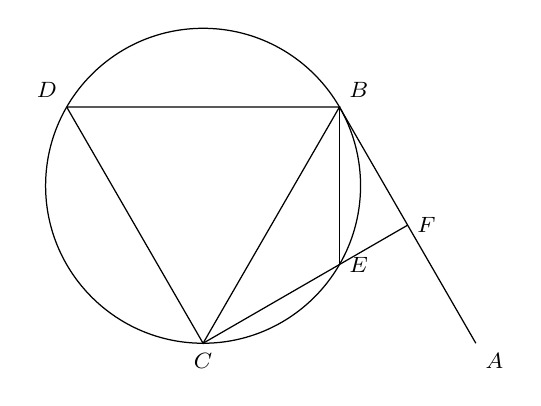
\begin{tikzpicture}[font=\footnotesize, line width=0.45pt]
  \coordinate (O) at (0,0); \coordinate (B) at ({sqrt(3)},1); \coordinate (D) at ({-sqrt(3)},1);
  \coordinate (C) at (0,-2); \coordinate (E) at ({sqrt(3)},-1);
  % F 为切线 sqrt(3)x+y=4 与 CE 的精确交点；A 在切线上。
  \coordinate (F) at ({3*sqrt(3)/2},-0.5); \coordinate (A) at ({2*sqrt(3)},-2);
  \draw (O) circle (2);
  \draw (D)--(B)--(C)--(D);
  \draw (B)--(E); \draw (C)--(F); \draw (B)--(A);
  \node[above right] at (B) {$B$}; \node[above left] at (D) {$D$}; \node[below] at (C) {$C$};
  \node[right] at (E) {$E$}; \node[right] at (F) {$F$}; \node[below right] at (A) {$A$};
\end{tikzpicture}
